\documentclass[10pt, a4paper]{report}
\usepackage[utf8]{inputenc}
\usepackage{lscape}   % Make a page in landscape format \begin{landscape}
\usepackage{colortbl} % To color table cells
\usepackage{color} % Able to change textcolor
\usepackage[table]{xcolor}
\usepackage{longtable}
\usepackage{graphicx} % Able to add pictures
\usepackage{parskip}  % Separate paragraphs with a blank line
                      % rather than using indentation
\usepackage{hyperref} % Support for hyperlinks
\usepackage[protrusion=true,expansion=true]{microtype} % Improve justification
\usepackage{subfigure}
\usepackage{hyperref}
\usepackage{caption}
\usepackage{float}
\usepackage{afterpage}
\usepackage{lipsum}
\usepackage{wrapfig}
\usepackage{enumerate}
\usepackage{natbib}

\hypersetup{%
    pdfborder = {0 0 0}
}

\begin{document}

	\begin{titlepage}
\begin{center}

	{\Huge ``Can You Keep a Secret?''\\ [0.4cm]
	- A study of Android Unlock Patterns} \\[1.5cm]

	%Can you keep a secret?
	%Tell me who you are, and I will know your password.

	{\Large TDT4501 - Project Thesis} \\[2.0cm]
	{\Large Marte Dybevik Løge} \\ [0.5cm]
	{\Large Norwegian University of Science and Technology}\\

	\vspace{3.0cm}

			
\includegraphics{pics/ntnu-logo2.png}

	\vspace{3.0cm}

	{\Large Submission date: Desember 2014} \\[0.2cm]
	{\Large Supervisor: Lillian Røstad} \\ [0.2cm]
	{\Large Co-supervisor: Per Thorsheim} \\ [0.2cm]
	{\Large Keywords: graphical passwords, mobile security, Android}


\end{center}
\end{titlepage}\clearpage
	\section*{Abstract}
  
  Since the first proposal for a graphical password around 1996, a variety number of graphical password schemes have been proposed. The proposed graphical password schemes were motivated by the promise of improved password memorability and thus usability, while at the same time trying increase the security.  Psychology studies have recognized that the human brain have a superior memory for recognizing and recalling visual information rather than recognizing and recalling verbal or textual information. Graphical passwords seems as a good replacement of text-based authentication. 

  The motivation for this thesis started by observing the shortcomings with text-based authentication, where people tend to obtain bad habits because of the difficulty of remembering the textual information. People therefore tend to create easily guessed passwords. Password sharing and password reuse are also some of the know habits that people obtain by using text-based passwords. When looking at mobile devices, text-based passwords are not easily typed on a mobile screen. Graphical passwords do not only seem as a good replacement of text-based passwords, but also look like a great authentication method for mobile devices because of the easily interaction with graphical elements on a small touch screen. Graphical passwords on mobile devices are used as a screen lock mechanism to prevent unwanted acess. The history of locking mechanisms was often a solution solely to prevent accidental use, while current mobile phones require protection in order to secure the potentially vast amount of private data that we keep on our mobile devices.

  Android Unlock Patterns is one of the graphical password schemes with an commercial success on mobile devices. The only large-scale study that have conducted quantified the security of peoples choice in patterns. This study aims to take the analysis of people's choice in Android Unlock Patterns a step further by including the human properties that may impact the user's choice in graphical passwords. I believe that graphical passwords are more than just pictures and graphical objects.

  In this thesis there is conducted a literature review of graphical passwords. There is also created a proposal for a research design for further continuation of this work. The research design contains a research strategy, as well as a prototype for data collection. 

  \clearpage
	\tableofcontents \clearpage
	
	%Chapter 1 - Introduction
	\chapter{Introduction}

\section{Background and Motivation}
    
  % In todays society we're addicted to our mobile devices in our every day life. Mobile devices are not just a communication tool for calling and texting, but also an important tool for every day tasks like doing our work, reading mail, pay our bills and keeping up with our social life. Our whole life is contained in one device! When such a small device is so imortant, it makes it vurnerable. How do we secure it?

  % %Information security have become a critical concern from a business point of view

  % There are many different security tips for mobile devices, but the most imortant of them is locking your device with a password. There are many different password schemes, but the most commonly used password schemes are PINs, passphrases and graphical passwords.

  % The interest in graphical passwords started by the assumption that pictures are easier to remember and more secure than words and numbers. Google's Android platform released the  functionality for Unlock Unlock Patterns in 2008. The Android Unlock pattern is a graphical password schemes that asks the user to make a pattern on a 3x3 grid by making a patten of connected nodes. Since its relese there have been a lot of discussion of its security, but few researchers have done a scientific reseach on this. The problem is not just the theoretical password space, but the password space in practice.

  % In 2013 a research group conducted the first large-scale user study on Android Unlock Patterns \cite{Uellenbeck}. The outcome of the research was a analysis of 2900 collected Android Unlock Patterns. They found a lot of bias in the pattern making process cocluding that the schemes are less secure than its theoretical security.

\clearpage
\section{Research Questions and Goals}

The aim of this project is to design an experiment for collecting graphical passwords set by different user types that further will be used in my master thesis the following spring. In the experiment it will be collected passwords, as well as information about the users creating the passwords. Before designing the experiment this thesis will include a detailed state-of-the-art study on passwords. In order to understand the human factors that impacts how people make their passwords, this thesis will also include a study of the psychological aspects that connects humans and passwords. This are covered in my research questions below:

  \subsection*{Research Questions}

    {\bf RQ1: What is the status of current research on graphical passwords? } \\
    Research are always moving forward with new hypothesises and new results in the field. In order to do a research is imortant to know the relevant work as well as avoid answearing questions that already have been aswered.
    
    {\bf RQ2: What human factors may affect our choice of passwords?} \\
    Passwords are human-chosen secrets that are only connected to you as a person. When the secret are created you might create a password that are a association to something you know or recognice; passwords are more than just words and numbers. It is important to study the bias introduced in the password making process that can be a cause of human factors. Psychology are a field of study that might can give a understanding of how we think and give an explanation of why we make the choices that we do. 
    
    {\bf RQ3: How should an experiment to collect graphical passwords set by varoius user types be designed?} \\
    It is important to consider the biases that can be introduced as a cause of the experiment design. The design have to consider what data that needs to be collected and how the data should be collected. It is also important to consider the diversity of the data in order to be able to get good resluts from the analysis. The result will be a detailed design on the experiment that will be conducted in the following spring. 

\section{Research Method}  

\section{Thesis structure}





% \item To what extent can graphical elements like colors, shapes, and objects infuence the end-users choice of passwords?
% \item How is features describing the end-user picked, and how do the features relate to end-user's choice of passwords?
% \item Kan grafiske elementer påvirke brukerens valg av passord?
% \item Hvilke kjennetegn ved en person kan gi utslag på valg av passord?
% \item Hvordan skal innsamling av passord skjer for å ivareta datasamlingens pålitelighet?

% \item To what extent can we relate existing research on users choice of alphanumeric passwords to users choice of Android unlock patterns? 
% \item How should passwords from end-users be collected in order to preserve the reliability of the data? 
% \item In order to analyse collected Android unlock patterns, how much data is needed to be collected, and how should the diversity of the data look like?
% \item What kind of data should be included in the data model?
% \item How should the data model be designed in order to cover relevant data for the analysis of the collected data?  
% \item What are the status on research on mobile security?
% \item How should passwords from end-users be collected in order to preserve the reliability of the data? 


	% Chapter 2 - BackgroundTheory
	  \chapter{An Introduction to Authentication Mechanisms}
  \label{chap:background}
  
    This chapter is an introduction to authentication mechanisms. Section~\ref{sec:authentication} is an introduction to the categorization of existing authentication mechanisms. The different authentication mechanisms will provide a description, as well as it attached benefits and drawbacks of using a particular authentication mechanism. Section~\ref{sec:entropy} provides an introduction to fundamental aspects of security and authentication. Section~\ref{sec:shortcomings} is an evaluation of the text-based authentication and its shortcomings.

  \clearpage

  \section{Authentication} \label{sec:authentication}

  Authentication is the process of verifying whether a particular individual or a device should be granted access to a system or application running on a device \cite{IPAS}, e.g. verifying that you are the person that you claim to be.

  There are various authentication schemes described in the literature, but they can all be grouped by the following characteristics:

    \begin{itemize}
      \item Who you are
      \item Something you have, and
      \item Something you know
    \end{itemize}

    \subsection{Biometric Authentication}
    Biometric authentication has the characteristics of ``who you are''. Biometric authentication refers to verify a person's identity based on physical or behavioral characteristics of an individual \cite{biometrics, biometrics2}. Biometric authentication is different from other authentications schemes because:

      \begin{itemize}
        \item the biometric password cannot be lost nor forgotten,
        \item biometric passwords tends to be difficult to copy, share and distribute, and 
        \item the person being authenticated needs to be present in the authentication process
      \end{itemize} 

    Physiological biometrics uses the physiological characteristics of an individual in the authentication process. The verification uses unique characteristics of a human, e.g. physical parts of the body that are unique as fingerprints, face, iris, hand and finger geometry, and DNA. Behavioral biometrics analyzes how a person performs different activities, e.g. applies pattern recognition techniques for activities like keyboard writing, talking and handwriting.

    The benefits achieved by using biometric authentication is that each password is unique and only connected to one person. When using an authentication scheme that requires the user to use something they know in the authentication process, it might be forgotten or shared. Biometric authentication cannot be shared, nor copied. The user does also not need to remember the biometric password because it is a part of you.

    There is also some drawbacks with biometric authentication. The implementation of biometric authentication is more complicated to implement because of the hardware needed. Other aspects of biometric authentication are the reliability. Many of the existing equipment used at, for instance, an airport only use images of the finger, and many do not detect if a real fingerprint is used. The same is used for face recognition where it is only used algorithms for authenticate the image of the face. In the case of fraud, you can categorize it as identity fraud because a part of you used for authentication is stolen. It is, therefore, a high responsibility for owners of a system using biometric authentication to store the data in a safe way.

    \subsection{Token-based Authentication}
    In a token-based authentication process the user uses ``something you have'' that is often stored on a physical device. Token-based authentication is often combined with a ``something you know'', making a strong authentication by combining two or more authentication characteristics. In many banking systems you have to use more than just something you know, but also ``something you have'', like a one-time password to pass the authentication process. The one-time password is a password that is generated on the physical device. This is an extra layer of security, because even if someone steals or know your password, he or she still can't get access to your banking account because he or she also would need your security token.

    One drawback of using token-based authentication is that the user must carry the token with them. Without the token, the users are not able to be authenticated. 

    \subsection{Knowledge-based Authentication}
    `Something you know'' is often used in the classical login situation where the user has to remember a username/password to get access to the system or device. Some of the commonly used passwords schemes are PIN's, alphanumeric passwords and graphical passwords that all are passwords with the characteristic of ``something you know''.

    One of the benefits by using knowledge-based authentication is that this is the authentication type that is mostly used for authentication. Since most systems use it, people are also familiar with how it works. The technical solutions do also not require any hardware and can be implemented at a low cost.

    One drawback is that the users needs to remember the password used in the authentication. Since the knowledge-based authentication is used in many systems, especially on Internet, the users are also required to remember all the various passwords on different systems. Requiring the users to remember the password often causes the users to select simple password that is easy to remember, and therefore might be easy to guess.

    There are three different knowledge-based authentication types:

    {\bf PIN's} Personal identification number is a numeric password. The PIN was first introduced in the first ATM in London in 1967 as an efficient way for the banks to authenticate their customers \cite{Bonneau1}. PINS are often a four-digit number. The benefit with a PIN is that it is a short sequence. The drawback is that people often tend to choose a sequence of number that are easily memorized. A known selection of PIN is to select a date that is easily remembered like the date of birth. Such choices are well known to attackers, and such PIN codes can easily be guessed.

    {\bf Alphanumeric passwords}
    The word ``Alphanumeric'' is a composition of the phrase ``alpha'' (as in alphabet), and ``numeric''(as in numbers). The alphanumeric password may also contain special characters, so in short an alphanumeric password is a mix of all writable characters. This is rapid used in systems using a combination of username and password. One drawback is that, like with PINs, people often choose a sequence of characters that is connected to the person. A know strategy for passwords selection is to choose words that are associated with the system, or words that are closely related to the person.

    Systems using alphanumeric passwords often requires the users to change the password at specified intervals. This often causes users to choose a simple password and only make a small change to the password when a change is required. If an attacker knows the password policy, it is possible to make a dictionary with likely used words and characters.

    {\bf Graphical passwords}
    A graphical password has the characteristics of ``something you know'', but instead of using letters and numbers it uses graphical elements. Graphical passwords were proposed as an alternative to PINs and alphanumeric values because humans tends to remember graphical elements better than letters and numbers. A variety of graphical passwords schemes has been created over the past years. Biddle et al. have collected research of the past decade on graphical password schemes \cite{Biddle}, dividing the schemes into three categories:

      \begin{itemize}
        \item Recall-based authentication
        \item Recognition-based authentication, and 
        \item Cued-recall authentication.
      \end{itemize}
      
    Recall-based graphical passwords are often referred to as drawmetric systems \cite{DeAngeli} because the user are are reproducing a secret drawing. The password is usually drawn in a grid or a blank canvas, requiring the user to reproduce the secret password from its memory.

    Recognition-based passwords are often referred to as cognometric systems \cite{DeAngeli} because the user recall a secret drawing or sequence of drawings.

    Cued-recall is often referred to locimetric systems \cite{DeAngeli}. With cued-recall authentication typically require the users to remember and target a particular location within and image. This is a version of a recall-based authentication but helps the user with the recall by showing an image and not just a grid or canvas. It is also different from the recognition-based approach because the user needs to identify specific locations in the picture as a whole. 
    
  \section{Key Security Aspects in Authentication} \label{sec:entropy}
  In order to be able to evaluate the security of different password schemes, this section will give a brief introduction to key security aspects of knowledge-based authentication, and hereafter called passwords. In terms of security, the primary goal of authentication is to provide protection for its intended environment in order to avoid security attacks. A password, regardless of format, is a secret a user needs to use in order to to grant access to the system or device. A password should have certain features in order to be secure:

    \begin{itemize}
      \item The password should be hard to guess, meaning that the password should have a high entropy,
      \item The password should be easy to remember for users, and 
      \item The password should remain a secret for the intended user.
    \end{itemize}

  When we talk about security, we often talk about if a password scheme is ``crackable'', meaning that the a password are guessable. When a password scheme is measured to be ``hard to guess'', it is normal to measure the strength of the password scheme in terms of its entropy. The password strength is measured in terms of information entropy, measured in bits. Instead of measuring the security of a password in number of guesses needed to guess the password, we use the base-2 logarithm of the number of guesses, which is the number of ``entropy bits'' in a password. We use the notation L for the length of the symbols in the password, and they are chosen from a set of N possible symbols. The formula for password entropy are:

    \begin{equation}
      Password Entropy = log_{2}(N^{L})
    \end{equation}

  When we say that a password scheme is easy to use it is normal to measure the success rate when writing and remembering a password, e.g. how long it takes for users to write and remember their passwords. When a password is easy to remember, it often refers to a password scheme ability to maintain its usability. As stated, a password that have a higher entropy are harder to guess, but are often obtained by making long passwords. It is well known that humans have a hard time remembering long and complex passwords. Therefore, it is important that a password scheme are supporting the users to make passwords that they can remember, and also are secure.

  When users make their password it should only remain a secret that the intended user know about. A password scheme that lack support of usability often make people do like create simple passwords that are easy to remember, but also easy to guess, or even write down and use the same passwords on multiple systems.

  All of the key security aspects are important to understand when you are studying password mechanisms. The fundamental aspects will be used throughout this thesis in order to be able to evaluate and read research focusing passwords. 

  \section{Shortcomings With Text-Based Authentication} \label{sec:shortcomings}

  User authentication is a central component of security systems. In order to get access to systems, you need to pass the authentication process. Despite the extensive number of options for authentication, text-based passwords remain the most common authentication scheme. The reason they are widely adopted is because they are easy and inexpensive to implement, and users are familiar with the scheme. It is also avoiding the privacy issues raised by biometric authentication and prevent the need for bringing a physical security device that are used in token-based authentication schemes. However, text-based authentication suffers from both security and usability disadvantages. Today, users needs to remember an increasingly number of password, making users adopt bad password habits.

  The term ``habit'' is often a bad thing when talking about security. A habit is often hard to change and are often a predictable pattern. Password reuse is one of the known password habits among users because the human limitation to remembering text-based password. Some users also make simple or meaningful password that are easier to remember, making their passwords vulnerable to attacks. It is a well-known problem that users tend to have an increasingly number of accounts that requires the users to remember yet another number of password on multiple systems and devices. The problem is not just to remember all the password needed, but also remembering which passwords that belong to which account or device. Because of the human capacity for remembering password are causing users to choose weak passwords, as well as reuse the passwords across multiple web pages. In order to understand the shortcomings with text-based passwords, this section will include relevant research on users choices on text-based passwords.

  Password schemes have what is called an empirical password space, and that is the number of possible passwords that a user can make. The problem with many password schemes is that it seems that users don't tend to use the full password space, but only a subset of the possible passwords, e.g. the memorable password space, making the memorable password space less than the empirical password space (Figure~\ref{fig:memorable}). This shows that the security of a password scheme is linked closely to is memorable password space rather than its full password space.

  \begin{figure}[H]
      \centering
      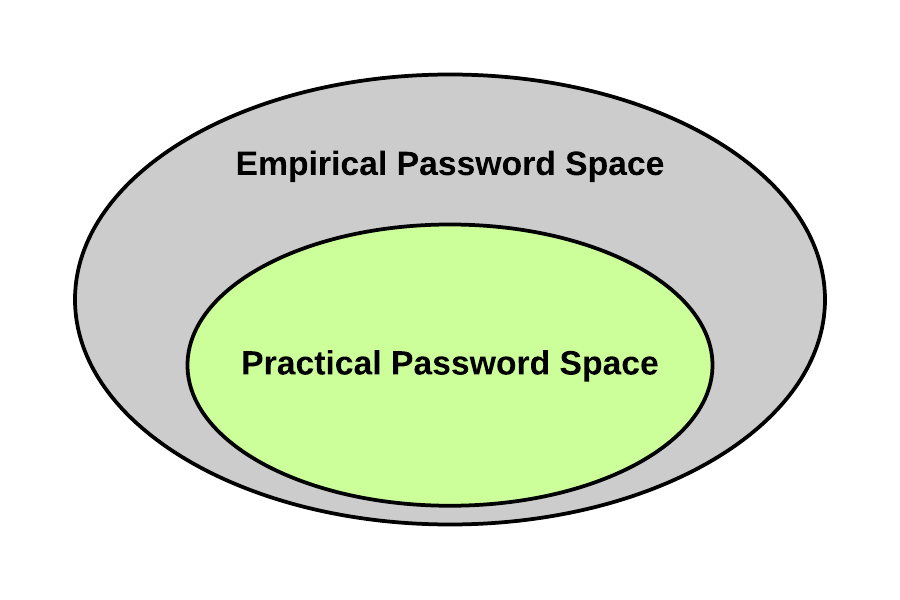
\includegraphics[scale=0.25]{pics/EmpiricalVsPractical.png}
      \caption{Empirical vs. Memorable Password Space}
      \label{fig:memorable}
    \end{figure}

  In a case study of 14.000 Unix passwords, a research group found a 25\% of the passwords were in a group of words forming a dictionary of $3\times10^{6}$ words \cite{UnixPasswords}. This dictionary shows that an attacker can have a relatively high success rate for an attack, despite the fact that there a roughly $2\times10^{14}$ 8-character passwords consisting of digits, and upper case and lower case letters. Due to the limitations of human memory, users often choose passwords that are easier to remember, causing a significant number of user-chosen password to fall into a small dictionary, e.g. practical password space \cite{Tao}. A well-designed dictionary is a tiny subset of the full password space, e.g. theoretical password space, which further can be prioritized according to the likelihood for a password to be chosen. It is, therefore, a commonly stated that the security of a password scheme is related closely to the size of its memorable/practical password space, rather than its theoretical password space. The high success rate of dictionary attack against textual passwords is believed to be strongly related to the recall capabilities of humans and how they choose their passwords, e.g. making meaningful and thus more easily remembered words are selected as passwords.

  One of the first large-scale studies on web password habits was conducted in 2007 by Microsoft research \cite{habits1}. They analyzed web password habits among 544960 Internet users over a period of 3 months. The data was collected from a Windows Live Toolbar, and they observed activities like login frequency. They also gathered information about the users age, the strength of the users passwords, as well as number of unique passwords and its use across different URLs. They observed that a typical user have an average of 7 distinct passwords and that an average of 5 of these passwords was re-used on different web pages. An estimate of the average number of account per user was estimated to be 25 accounts per user, but this would probably be higher since it seven years ago.

  Because of the shortcomings with a text-based authentication, graphical authentication are getting increased attention because it is an alternative to a text-based authentication trying to cope with the memorability and security issues of text-based password. Graphical passwords are using images and visual objects in the authentication instead of text and numeric values. When comparing text against visual objects, the human brain is more capable of remembering images than text. When the human brain is more suited for remembering images, the users might be able to remember more complicated passwords that are not easily guessed. To context where an authentication scheme is used have to be evaluated. Graphical passwords might not fit in all systems, but looks like a good alternative to mobile devices where the user interact with a touch sensitive screen. Typing a long text-based password on a small keyboard on a mobile device is not easy. When using, graphical passwords are easier to interact with on a small mobile screen.


	% Chapter 3 - Litterature Study
	
\chapter{Litterature Review}

	{\bf \color{red} Write introduction}

  % Utfordringen med passord
  % Hvorfor er ikke passordtypene vi har gode nok?

  % Hva betyr det at et passord er knekkbart?

  % hvorfor er dette med passord et viktig tema som man enda ikke anser som løst?
  % ---> Menneskelige faktorer i sikkerhetssammenheng

  % - Det jeg savner at du skriver noe om er utfordringen med passord. Hva søker man etter når man lager nye passordmekansimer? (entropi, vanskelig å gjette, lett å huske etc). Hvorfor er ikke de typene vi har gode nok? Hva betyr det at et passord er knekkbart? Kort oppsummert: hvorfor er dette med passord et viktig tema som man enda ikke anser som løst?

  

  


	\section{Shortcomings With Text-Based Authentication} 

  %\cite{DejaVu}
  User authentication is a central component of security systems. In order to get access to systems you need to pass a authentication process. Despite the large number of options for authentication, text-based passwords remain the most common authentication scheme. The reason why they are widely adopted is because they are easy and inexpensive to implement, and users are familiar with the scheme. It is also avoiding the privacy issues raised by biometric authentication and avoid the need for bringing a physical security device that are used in token-based authentication schemes. However, text-based authentication suffer from both security and usability disadvantages. Today, users needs to remember an increasingly number of password, making users to adopt bad password habits. 

  The term ``habit'' is often a bad thing when talking about security. A habit is often hard to change and are often a predictable pattern. Password reuse is one of the known password habits among users because the human limitation to remembering text-based password. Some users also make simple or meaningful password that are easier to remember, making their passwords vulnerable to attacks. It is a well known problem that users tends to have an increasingly number of accounts that requires the users to remember yet another number of password across multiple systems and devices. The problem is not just to remember all the password needed, but also remembering which passwords that belongs to which account or device. Because of the human capacity of remembering password are causing users to choose weak passwords, as well as reuse the passwords across multiple web pages. In order to understand the shortcomings with text-based passwords, this section will include relevant research on users choices on text-based passwords.  

  \begin{wrapfigure}{l}{0.4\textwidth}
    \vspace{-20pt}
    \begin{center}
      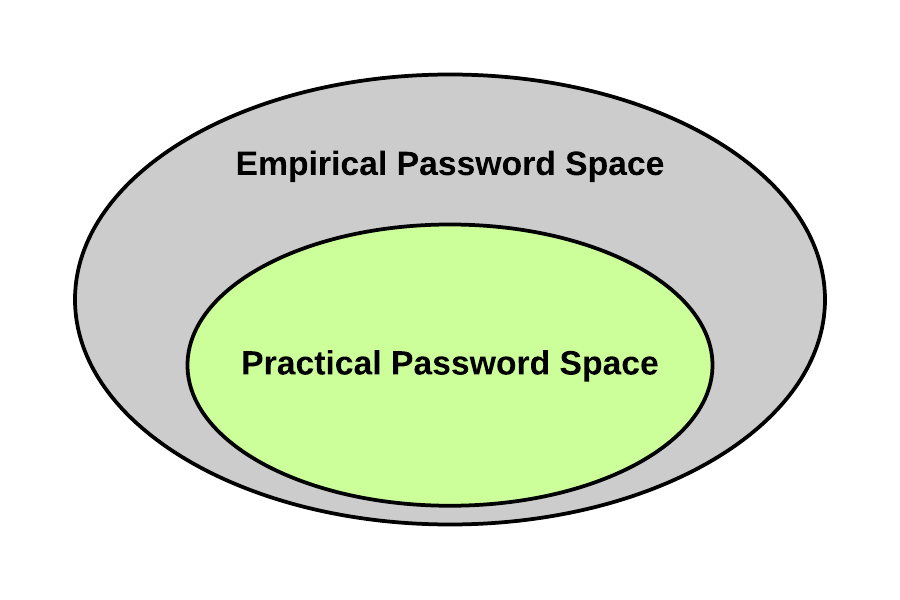
\includegraphics[scale=0.16]{pics/EmpiricalVsPractical.png}
    \end{center}
    \vspace{-20pt}
    \caption{Empirical vs. Memorable Password Space}
    \vspace{0pt}
  \end{wrapfigure}

  Password schemes have what is called an empirical password space, that is the number of possible passwords that a user can make. The problem with many password schemes is that it seems that users don't tend to use the full password space, but only a subset of the possible passwords, e.g. the memorable password space, making the memorable password space less than the empirical password space. This shows that the security of a password scheme is linked closely to is memorable password space rather than its full password space. 

  In a case study of 14.000 Unix passwords, a research group found a 25\% of the passwords were in a group of words forming a dictionary of $3\times10^{6}$ words \cite{UnixPasswords}. This dictionary shows that an attacker can have a relatively high success rate with an attack, despite the fact that there a roughly $2\times10^{14}$ 8-character passwords consisting of digits, and upper case and lower case letters. Due to the limitations of human memory, users often choose passwords which are easier to remember, causing a significant number of user-chosen password to fall into a small dictionary, e.g. practical password space \cite{Tao}. A well-designed dictionary is a tiny subset of the full password space, e.g. theoretical password space, which further can be prioritized  according to the likelihood for a password to be chosen. It is therefore a commonly stated that the security of a password scheme is related closely to the size of its memorable/practical password space, rather than its theoretical password space. The high success rate of dictionary attack against textual passwords is belived to be stronly related to the recall capabilities of humans and how they choose their passwords, e.g. making meaningful and thus more easily remembered words are chosen as passwords. 

  One of the first large-scale studies on web password habits was conducted in 2007 by Microsoft research \cite{habits1}. They analyzed web password habits among 544960 web users over a period of 3 months. The data was collected from a Windows Live Toolbar and they observed activities like login frequency. They also collected information about the users age, the strength of the users passwords, as well as number of unique passwords and its use across different URLs. They observed that a normal user have an average of 7 distinct password and that an average of 5 of these password was re-used on different web pages. The estimate on average number of account pr user was estimated to be 25 account pr user, but this would probably be higher since it 7 years ago. 

  {\color{red} \bf WRITE SOMWTHING MORE??}

  %REWRITE!!!
  Because of the shortcomings with text-based authentication, graphical authentication are getting getting increased attention because it are an alternative to text-based authentication trying to cope with the memorability and security issues of text-based password.
   

	\section{Graphical Passwords}

% Må få frem hvilke grafiske passord som er laget, samt se på hvilke problemer de løser/ikke løser
% Kommentar fra Lillian: Hva søker man etter når man lager nye passordmekanismer? (entropi, vanskelig å gjette, lett å huske)

  Like text-based passwords schemes, graphical password schemes are also a knowledge-based authentication scheme, e.g. ``something you know'' that are described in the background theory. Since it all started around 1996, there have been many suggestions for graphical password schemes. When a new password scheme are proposed, there are several aspects of password that needs to be considered. A password scheme needs to be secure in terms of entropy, it needs to be hard to guess and it also needs to be easy to use. This section will give a brief introduction to the history of research published on graphical passwords. This is important to know because each scheme is trying to improve different aspects of graphical password, giving us a detailed understanding of todays situation. 

  The idea of graphical passwords was originally described by Greg Blonder in 1996 \cite{Blonder}. The graphical password scheme proposed was requiring the users to tap on a selection of points on a predefined image in order to pass the authentication process. This was just a proposal, and did not further explore the power of graphical passwords, nor analyzed the security aspects of the proposal. 

  In 1999, Jermyn et al. \cite{Jermyn} suggested a new graphical password scheme called ``DAS'' (Draw-a-secret). Draw-A-Secret (DAS) was the first recall-based graphical password scheme proposed. The motivation for the graphical password scheme was that graphical input devices enables the user to decouple the position of inputs from the temporal order in which they occur, and shows that the decoupling can be used to generate passwords that have a larger and more memorable password space. In order to make a more memorable password, the research group argued that the DAS was more secure than text-based passwords because the users were able to remember longer and more complex passwords. After the DAS scheme was published, Dunphy and Yan \cite{BDAS} added an extra background image, called ``BDAS'', in order to encourage their users to make more complex passwords.

  In 2000, Dhamija and Perrig \cite{DejaVu},created a new password scheme called ``Deja Vu''. The password scheme was based on the hash visualization technique \cite{HashVisualization}. The users are asked to select a sequence of images from a random set of images that are generated by a program. They wanted to make a graphical password scheme that solved some of the shortcomings with recall-based authentication like PIN's and text-based passwords. Deja vu should purely rely on recognition rather than recall, and it should be hard to write down and share the password with others. The randomly generated pictures based on the hash visualization technique makes it hard to share the password since the pictures is hard to recreate, but are easy to remember. 

  ``Passfaces'' is a graphical password scheme developed by Real User Corporation that was founded in 2000 \cite{passface}. The authentication procedure allows the users to first select four images that are a visualization on human faces, and the user get authenticated by identifying their four faces. The scheme exploits the advantage that people are good at recognizing people, so when users choose the human faces, they can recognize the characteristics of the faces.

  In 2002, Goldberg et al. \cite{PassDoodle} tried to make a graphical password scheme that combined both text an images called ``PassDoodle''. This is a graphical password combined of handwritten text. Their study concluded that users were able to remember complete doodle images as accurately as text-based passwords.

  In 2004, Davis et al. did a comparison of a light version of the ``PassFace'' and a new graphical password scheme called ``Story'' \cite{Davis}. The Story scheme is making the users choosing images making a story. The background for the scheme was to support their users of remembering their passwords by making a memorable story of images. The story that was made were needed to be recalled in a correct order. To aid memorability, users were instructed to mentally construct a story to connect the everyday images in the set. 

  In 2005 Wiedenbeck and Blonder made a graphical password scheme called ``PassPoints'' \cite{PassPoints} that is an  extension of the Blonder's \cite{Blonder} idea by eliminating the boundaries and allowing arbitrary images to be used. They evaluated their password scheme by testing the scheme on human users. The results showed that PassPoint were a promising scheme with respect to memorability because of the low error rate and low clicking rate. 
  The aim of this study was to get an understanding of how different images affected user performance in authentication with a graphical password scheme. The preliminary result showed suggested that images may support memorability in graphical password schemes. 

  In 2006, a research wanted to address the problem with graphical passwords and the shoulder surfing problem. They called their password scheme ``Convex Hull Click'' (CHC) \cite{Wiedenbeck} that allows the user to prove knowledge of the graphical password in secure and insecure location because they made the scheme in a way that users don't directly click on their password images, making it hard for attackers to do perform shoulder surfing. In CHC the windows shows a list of small icons. In the authentication process, the user needs to recognize some minimum number of their chosen password images, or ``pass-icons'', out of a large number of randomly places icons. This step are presented in a sequence, and if the user responds correctly every time, the user pass the authentication.
  
  In 2007, Tao and Adams \cite{Tao}, created a new proposal for a new graphical password scheme called ``Pass-Go''. The Pass-Go scheme is inspired by the old Chinese game, Go, where users selects intersections on a grid to maker their password. This was one of the first largest user studies on graphical passwords, and was made in order to improve the usability of graphical passwords. They try to emphasize that the usability of a graphical password scheme will increase the memorability of graphical password, causing the password scheme to be more secure.  

  Graphical passwords are also implemented on mobile devices, like the ``Android Unlock Pattern'', that is an mini version of the ``Pass-Go'' deployed on Google Android smartphones. ``PatternLock'' is a similar system that are available for Blackberry. Rather than entering a 4 digit PIN or a text-based password, the user enters a touch-drawn password on a $3\times3$ grid.

  Graphical passwords are still not widely adopted, but there are still new graphical password scheme being proposed. Recently published  graphical password schemes are GeoPass \cite{GeoPass} and Picassopass \cite{PicassoPass}. Geopass is uses a digital map for the authentication phase, where the user chooses a specific location as their password. Picassopass is a graphical password scheme that are presenting a password using a dynamic layered combination of graphical elements. The users can make a story that assists the user in the recognition of the graphical elements.

 \section{Evaluation of Graphical Password Schemes}

  \begin{wrapfigure}{l}{0.35\textwidth}
    \vspace{-20pt}
    \begin{center}
      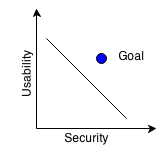
\includegraphics[scale=0.7]{pics/UsabilityVsSecurity.png}
    \end{center}
    \vspace{-20pt}
    \caption{Usability vs. Security}
    \vspace{-10pt}
  \end{wrapfigure}

  Authentication with text-based passwords are a common approach, but it is well known that users often choose weaker passwords because of the limitations of recalling text-based passwords. Graphical passwords came as an alternative solution for overcoming the limitations of text-based passwords, and was inspired by researchers that showed that the graphical memory of humans is particularly well-suited to remember graphical information \cite{DeAngeli}. The problem with many graphical password schemes is that they often promise improved password memorability and thus usability, while at the same time improving the security \cite{Biddle}. This is why it is important to understand both the usability and security aspects when looking at different password schemes in order to understand the trade off between different design choices.

\subsection{Usability and Memorability}

  \todo{Finne forskning som evaluerer grafiske password på usability and memorability}

  An interesting question is what classes of graphical password users find memorable. Based on cognitive studies of visual information, Oorschot and Thorpe \cite{Thorpe1} investigated the memorable password in the graphical password scheme DAS \cite{Jermyn}. They found that the were less or equal to the length of 8 on a 5$\times$5 grid. This results compared to textual passwords may offer greater security against dictionary attacks. 

  If the number of possible pictures in a graphical password scheme is large enough, and the diversity of the of picture based passwords can be captured, it seems reasonable to argue that memorable password space of a graphical password scheme will be higher than text-based password schemes, making graphical passwords offering better resistance to dictionary attacks.
  When the proposal for the graphical password scheme ``Deja Vu'' was proposed, they did a user study that showed that 90\% of all participants succeeded in the authentication tests using Deja Vu while only about 70\% succeeded using pass words and PINS \cite{DejaVu}. This is an example that users tends to have a higher success rate remembering graphical password, rather than text-based passwords. 

  One of the first graphical password schemes, ``DAS'' \cite{Jermyn}, offers a theoretical space that are comparable with text-based passwords, but results from research shows that users tends to draw symmetric images with few pen strokes, and often place their drawings in the center of the grid. The ``BDAS'' scheme \cite{BDAS} tried to avoid this by adding a additional background image, and the results showed that it reduced the amount of symmetry within password images, and supported the users to make longer passwords that were similarly memorable as for the ``DAS''. It remains still a problem that many of the research published on graphical passwords are preformed with a pen and paper approach, raising a question about the validity of the results. One problem may be that many graphical passwords are not implemented, but only a theoretical suggestions. It still remains a lot of research on graphical passwords in their intended environment. 

  Davis \cite{Davis} did a comparison of the memorability between the graphical password scheme ``Face'' (a light version of the ``PassFaces'') and ``Story''. This results reported that users had more difficulty remembering Story password (success rate of 85\%), mostly of the errors was introduced because they had to remember the correct sequence of the images. 

  When looking at usability we can evaluate the graphical layout of a graphical password scheme to see if the visual elements impacts the users choice of passwords. Ullenbeck et al. \cite{Uellenbeck} looked at the Android Unlock patterns and investigated if a change in the graphical layout would impact the security. The Android Patten Lock is made on a 3$\times$3 grid of connected points. Instead they rearranged the points in 4 different positions and analyzed collected data. The results showed that they managed to double the password space by rearranging the points and reduce the biases that are found in the original position of the nodes, but also introduce new ones. One of the rearrangements was a random approach. Unfortunately, this random arrangements of nodes looked like the mathematical ``delta'', so many people recognized the symbol. The random arrangement scored the worst entropy since many of the user chose the same pattern. They did not have several recognizable arrangements, but since people are good at recognizing and memorize patterns, it would not be surprisingly if they would find the same results in other rearrangements that was similar to a user-known symbol.  

  Wiedenbeck et al. \cite{Wiedenbeck1, Wiedenbeck2, Wiedenbeck3} conducted three lab-based user studies of the graphical password scheme ``PassPoint''. The results showed that the users needed an average time of 63 seconds in order to create their password, and an additional average time of 171 seconds in training time in order to remember the password. The login time took an average time of 9 and 19 seconds. This highlights important research of usability and memorability of a graphical password scheme. Some of the factors that makes a password scheme to have hight usability is deiced by average creation time, time to remember the password, as well as time used in the login phase. 

  \todo{Legge til forskning på usability av pass-go}

    
\subsection{Security}

  In knowledge-based authentication, e.g. ``something you know'' we classify attacks into two general categories: guessing and capturing attacks. In a guessing attack the attackers are able to search through the entire password space, or either predict the users passwords patterns in order to avoid searching through the whole passwords space (often referred to as a dictionary attack). This is often associated with the entropy of the password, because the lower the entropy it will be easier to make a successful attack. When talking about capturing attacks, the attackers are able to directly obtain the passwords by observing the authentication process. One of the known capturing attacks on graphical passwords are shoulder surfing because of its graphical visualization.  

  Since a person needs to remember a password, it is normally to choose a password that are connected to you as a person in order to remember the password, causing the password to have bias. A bias can be explained as a prejudice in favor of or against one thing, person, or group compared with another, usually in a way that influence a person choice of action. Since psychological studies have recognized that the human brain have a superior memory for recognizing and recalling visual information, it support the statement that users are able to remember more complex graphical password form a larger password space than a alphanumeric password. Logically the attacker then have to build a bigger and more complex dictionary, thus spend more time to achieve the same success rate as for textual passwords. 

  The graphical password scheme DAS \cite{Jermyn} was evaluating the security of their password scheme. They highlighted that there are many factors that impacts the security of a password scheme, like the statement that the users do not use a uniform distribution of all possible passwords, using Klein's study \cite{UnixPasswords} as a argument. The fact that users do not pick passwords uniformly is not in itself a sufficient statement to make a guessing attack successful. They try to cover the possibility for a attacker making a successful attack by making their scheme complex, and the results showed that the generated passwords was significantly harder to crack in practice than textual passwords. The problem is that they used computer generated passwords that will not show actually password chosen by user. They did not analyze the security of the DAS including human factors and password biases that may could influence the practical password space. 

  There is a lack of analysis on graphical password on users choices in graphical passwords. Davis et al.\cite{Davis} evaluated the security of the ``PassFace'' graphical password scheme. They found that there was a bias that was introduced by the demographics of the users. The users tended to choose faces that they liked and could compare themselves to. The results showed that if you knew the gender and race of a user, you could perform a dictionary attack to guess users passwords. If the gender of a user was known as male, then 10\% of the passwords can be easily guessed on the first or second attempt. Similarly, if the race of a user was known to be Asian and his/her gender is known, then 10\% of the worst passwords can be guessed within the first six attempts. The results indicated that the human passwords was heavily biased, and they stated that the graphical password scheme was insecure. 

  Dirik et al. \cite{Dirik} conducted an experiment by modeling user choice in the graphical password scheme ``PassPoints''. The aim of this study was to test if it was possible to build a dictionary attack based on users choice in clicking points. In this study they predefined two different images with a different level of salient points. The results stated that they could recover 61\% of the users passwords by searching through a smaller password space that was based on a analysis of collected click-points. Normally, the ``PassPoints'' scheme provides user chosen password, but the aim of this study was to investigate if it was possible to predict users password in a dictionary attack. There was a slightly difference in the two images that the researcher picked, where the image with less salient points was stated as insecure. Since the ``PassPoints'' scheme ables the users to pick their own password, the security may relay on the chosen image by the user and not the scheme by it selves. The results from this research can not it selves state that the ``PassPoints'' scheme is insecure, but highlights that it is important to consider the human factors in security because it may influence the total security in a graphical password scheme. 
  The same year another research group published \cite{Thorpe2} results on security of the ``Passpoints'', but using different approaches. They conducted a user studies to test if it was possible to make a offline attack, as well as using a image-processing tool for simulating a offline attack on the same images that were used in the user studies. They provided empirical evidence that popular points, e.g. hot-spots, do exists in images. The results from the most effective attack was generated by harvesting passwords from users to attack other targets. The probability for the guessing attack showed that 36\% of the passwords selected by users could be guessed within $2^{31}$ guesses and 12\% within $2^{16}$ guesses. The results from the offline attack using image-processing were slightly less effective, but they still managed to prove that a offline attack is possible to use on graphical passwords.   

  \todo{Her må jeg ha med flere eksempler på forskning som fokuserer på angrep}

  In one of the first large-scale studies on the Android Pattern Lock \cite{Uellenbeck}, they stated that the entropy of patterns is rather low, and the results from the study indicated that the security offered is less than the security of only thee digits randomly assigned PIN for guessing 20\% of all passwords. In the same research they made a Markov model based on collected passwords from users categorized as offensive and defensive patterns in their user study. The results showed that within 10 guesses they could guess approximately 4\% of pattern in the category defensive patterns and approximately 7\% of the defensive patterns. When increasing the number of guesses to 30 attempts, they managed to guess approximately 9\% of the defensive patterns and approximately 19\% for the offensive patterns. If we look further into the Android Unlock Pattern it have nearly 400.000 possible patterns, and are from a theoretical point of view stronger than a 5-digit randomly assigned PIN. The researchers evaluation of user chosen pattens shows that they only have an estimated entropy slightly lower than a 3-digit randomly assigned PINs. Another interesting result is the memorable password space used, where about 10\% of all users use less than 190 patterns, while less than 300 patterns capture around 50\% of the whole test population. This shows that a empirical password space are not a representative number when quantifying the security of a password, but we should look at the memorable password space, e.g. password that actually are used and memorable. The aim of this study was to close gap of lacking research on the practical password space on graphical passwords. 

  A clever attacker would narrow down the password space and prioritize guesses to pictures that people are likely to choose as a password. The images that are chosen are likely to be the pictures that users are likely to recall. In order to understand how an attacker might take advantage of human password choices, psychological studies on humans visual memory are important to understand. 

\clearpage
\section{Psychology and Human Factors}

  \begin{wrapfigure}{r}{0.35\textwidth}
    \vspace{-20pt}
    \begin{center}
      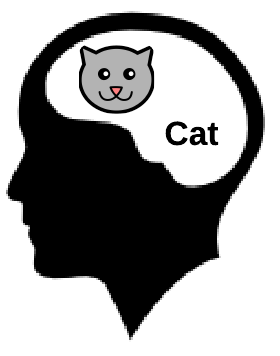
\includegraphics[scale=0.35]{pics/dualCoding.png}
    \end{center}
    \vspace{-20pt}
    \caption{Dual-Coding Theory}
    \vspace{-10pt}
  \end{wrapfigure}

  In many years, the field of psychology been a important in order to understand how humans interpret and remember different information. Psychology studies have recognized that the human brain have a superior memory for recognizing and recalling visual information rather than recognizing and recalling verbal or textual information \cite{DeAngeli}. One known theory is the ``dual-coding theory'' \cite{Biddle}, suggesting that verbal and non-verbal memory are processed and represented differently in humans mind. Text are verbal information that is represented symbolically, in contrast to non-verbal information like images that are mentally represented in a way that perceived concepts are assigned to a perceived meaning of what is directly observed. Both verbal and non-verbal information can be used when recalling information. For example, say a person have received stimulus of the concept ``cat'', both the image of a cat as well as the word ``cat''. When the person is asked to recall the concept ``cat'', the person can retrieve the image or the word individually, or both simultaneously. If the word ``cat'' is recalled, the image of the cat is not lost and can still be retrieved at a later point in time. The ability to code a stimulus in two different ways can increase humans ability to remember, in contrast to only code the stimulus in one way. In the background theory there are described three different categories of graphical passwords according to the memory task involved in remembering and entering the password, e.g. recall, recognition and cued-recall. 

  When it comes to humans and visual interpretation, studies supports the idea that people recall symmetric images better than asymmetric images \cite{Attneave, French}. A particular interesting observation is that mirror symmetry carries a special status i the human memory \cite{Wagemans1}. A understanding of psychological studies on humans visual memory can help to build successfully attacks against graphical passwords. If an attacker can successfully use the symmetric properties of graphical password schemes, then the security may be significantly less than if all passwords were equivalent probable. 

  Humans do not only tend to choose symmetric passwords, but do also tend to be influenced by the graphical elements in a password scheme. A study on ``PassFace'' \cite{Davis} showed that there was a high bias in the password selection according to a users gender and race. When they analyzed how each gender choose their password, the most of the male and female participants chose female faces, and and 60-70\% of the user chose a model over a typical female/male. They also looked into the race of the faces, where the results showed that almost all of the participant chose their own race. This research raise the question if it is possible to analyze users choice in passwords based on the demographics of the user.

  A difference in graphical and text-based password schemes is that graphical passwords are able to use images with colors that may influence the users choice in graphical passwords. In a user-study \cite{Thorpe2} on the image-based graphical password scheme ``PassPoints'' managed to see that different images were easier guessed than other images. When analyzing different images and visualizations we can look at studies of gestalt psychology \cite{Wagemans2} that uses the gestalt principles to understand users interpretation of a picture. One of the images that was the easiest to guess in the user-study was a image with cars in different positions in different colors. A possible explanation could be that humans seeks to find pattern that are easily remembered by using the like the principles of grouping, similarities of color, and similarity of size in image analysis.
  \todo{Legge til studier fra psykologi som kan forklare hvordan mennesker ser på sammensetningen av et bilde (cognitive studies)}

  There is a lot of studies on password based on psychology and human factors, but the graphical passwords schemes being analyzed do not look at the background of the users. Humans are different in terms of their demographics, like gender, age and culture in their country. Analysis of people choices of graphical password based on users background have not been looked further into in published research as based on this state of the art research. Since there is a lack of this on graphical password, we will take a look into people choices on text-based passwords based on human properties. 

  %Password habits in subpopulations
  Password habits may be different across different subpopulation in cause of different background or culture. In 2012 Joseph Bonneau released a analysis of 70 million passwords from Yahoo! \cite{Bonneau2}. The data is analyzed in terms of guessing rate by using a dictionary attack. The collected data contained 328 subpopulations. The results showed that there was no ``good'' populations among the collected data, but there was a variation in the population. Demographically, the gender had a small effect in the guessing rate, but it showed that age tended to give effect where password strength increases across different age groups. The analysis also showed that language had a significantly effect on the password strength where Indonesian-speaking users were among the weakest subpopulations, and in contrast the German and Korean-speaking users provided relatively stronger passwords. 

  \todo{Legge til mer forskning}
  

  \section{Graphical Passwords and Mobile Devices}
  %Intro
  Users are not only dependent on remembering passwords across multiple web pages and systems, but do also need to remember passwords for our small mobile devices. The mobile phone have emerged as a good platform for graphical passwords because it is easier to input on touchscreen as a contrast to text-based passwords. Graphical passwords on mobile devices seems as a natural fit, as they often require direct manipulation of visual elements. In todays society we're addicted to our mobile devices in our every day life. Mobile devices are not just a communication tool for calling and texting, but also an important tool for every day tasks like doing our work, reading mail, pay our bills and keeping up with our social life. This trend makes our mobile devices vulnerable in terms of security. To avoid unwanted access, smartphones offers different locking mechanisms. The history of locking mechanisms was often a solution solely to prevent accidental use, while current mobile phones require protection in order to secure the potentially vast amount of private data that we keep on our smartphones. The situation of our rapidly use of mobile phones, as well as it well suited platform for graphical password, makes authentication on mobile devices an interesting field of study.

  When looking at mobile security it essential to be familiar with the magnitude of mobile phone usage. As of 2014, over 90\% of American adults owns a mobile phone, whereas 58\% of American adults owns a smartphone \cite{MobileUseage}. Another 34\% of the users used mostly their phone to go online instead of using other devices such as a desktop or laptop computer. This is numbers from USA, but it still provides insight into the how common mobile phones is today.

  % Awareness about the sensitivity of the data stored mobile phones
  As stated earlier, smartphone user's tends to store sensitive information on their phones, it is therefore important to understand the relationship between the use of security features and users risk perceptions. One of the key security aspects on mobile phones that is important to understand is why people use or not use locking mechanisms on their smartphone. Engelman et al. \cite{Egelman} published a research paper in cooperation with Google on peoples smartphone locking behavior and attitudes towards security of their smartphone data. They observed a strong correlation between use of security features and risk perceptions. They reported that 33\% of the smartphone users were thinking about the locking mechanisms as too much of a hassle, while 26\% of the user's didn't think that someone would care about the information stored on their phone.  Other reported results have covered that the 46.8\% of the participants agreed or fully agreed that unlocking their phone can be annoying, but at the same time 95.5\% of the somewhat or fully agreed that they liked the idea that their phone was protected \cite{habits3}. A study reported that 29\% did not lock their smartphones \cite{MobileUseage}, while another research stated that among 35\% of mobile users don't lock their phone \cite{Bruggen}. The number may vary because of the background and experiences with security , but the number still remains quite high. This highlights that the users wants to be secure, but there might be a trade-off between the time used to unlock the smartphone vs the security risk. 

  % The time used on unlocking the phone
  In terms of security it is interesting to look at the use of mobile devices and look at the locking habits among users on mobile devices. It is known that services that are rapidly used have weaker password because of the overhead the user needs to spend on typing their password. In 2014 a group of researchers published a field study of smartphone (un)locking behavior \cite{habits3}. Some of the problems with smartphone users tends to be their rapidly use of their phone. When the device are rabidly use, it results in a lot of time unlocking their phone between every use. In the study they found that there was a significant overhead in the time used of unlocking their phone, where the users participated in the field study used 2.9\% (9\% in the worst case) of their time unlocking their smartphone. 

  It is stated that a lot of user's use their smartphones to perform tasks that involve use and storage of sensitive data. Smartphones in use today do not require their users to have a locking mechanism on their smartphone. It is well known that users tends to choose to easiest way out and may result in the choice of not having any locking mechanism at all. Based on the result of the overhead in time used on unlocking their phone, a result may be to take the easiest way out by ignoring the vulnerability of not using a locking mechanism at all. It have been discovered that over 40\% of the users only used a basic ``slide-to-unlock'' mechanism on their smartphone, as well as over 16\% didn't use any locking mechanisms at all \cite{habits3}. This highlights a major bad habit among mobile users. What happens if your mobile is stolen? A loss of a mobile phone is not just the cost for replacing the phone, but also a loss of sensitive data. If the phone is found by the wrong persons, the sensitive data on the phone may be lost and used for unintended purposes. A 2012 report from Pew Internet estimated that nearly a third of cell phone users have had their device stolen or lost \cite{StolenLost}. It is interesting to comparing peoples locking behavior towards phones that are stolen or lost. The same report also reported that 12\% of cell owners say that another person have accessed their phone, making the owners feel that their privacy have been exposed to the public.

  Beside loosing a physical device, what consequences are users exposed to? One point of attack is a persons email. If you can grant access to someones email, you probably can get access to a lot more. In a study reported that all of their interview participants had their email account automatically logged in, as well as 31\% of them did not use any locking mechanism at all \cite{Egelman}. The same research group investigated how much information you could gain from getting access to a persons email account. The results showed that both users with or without locking mechanisms found sensitive information in their email account like SSN, Bank Account Number, Email Password and Home Address.

  One of the popular password schemes on smartphones are the Android Unlock pattern. It is a graphical password scheme that have been shown to have biases when the password are user-chosen. A research group did one of the first large-scale user study on the security of the Android Unlock Patterns in order to quantify its security \cite{Uellenbeck}. They analyses the biases introduced in the pattern making process and added changes to the scheme in order to avoid the known biases in the password scheme. The researchers found that there is a high bias in the pattern selection process, e.g. the upper left corner and three-point long straight lines are very typical selection strategies. If the patterns was uniformly chosen, the probability of starting in at any point should be 11\%. The results showed that there was a strong bias of the starting point towards the corners. If the points were uniformly chosen, the probability for all four corners should be 44\%, but the results showed that the probability is close to 75\% in the pen-and-paper study. In contrast to this, the center point, the right, the upper, and the lower center points only get a probability of 14\% based on the results. Other results from the pen-and-paper study found that the average pattern length was 5.63 (with a standard deviation of 1.5). By looking further into the pattern length chosen by users, this is not a surprisingly result because this looks quite familiar with restriction of the Android Pattern Lock that requires the users to make a pattern of at least 4 connected points. As stated earlier, users tends to take a easy way out, making users choose short patterns that are easy to remember and type. Besides the pen-and-paper study, there was also conducted a user study that also showed a high bias towards the upper-left corner that had the bias of 43\% in the user study, and 38\% in the pen-and-paper study. This is supporting the researchers claim that users tends to choose less secure patterns ``in the wild''. 

  The way that the mobile phone is held, the size of the screen may also impact the way that people write their passwords, but this may need further research to answer.

  

	\section{Evaluation of Graphical Password Schemes}

  \begin{wrapfigure}{l}{0.35\textwidth}
    \vspace{-20pt}
    \begin{center}
      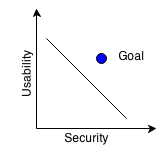
\includegraphics[scale=0.7]{pics/UsabilityVsSecurity.png}
    \end{center}
    \vspace{-20pt}
    \caption{Usability vs. Security}
    \vspace{-10pt}
  \end{wrapfigure}

  Authentication with text-based passwords are a common approach, but it is well known that users often choose weaker passwords because of the limitations of recalling text-based passwords. Graphical passwords came as an alternative solution for overcoming the limitations of text-based passwords, and was inspired by researchers that showed that the graphical memory of humans is particularly well-suited to remember graphical information\cite{DeAngeli}. The problem with many graphical password schemes is that they often promise improved password memorability and thus usability, while at the same time improving the security \cite{Biddle}. This is why it is important to understand both the usability and security aspects when looking at different password schemes in order to understand the trade off between different design choices.

\subsection{Usability and Memorability}

  {\color{red} \bf Finne forskning som evaluerer grafiske password på usability and memorability}

  An interesting question is what classes of graphical password users find memorable. Based on cognitive studies of visual information, Oorschot and Thorpe \cite{Thorpe} investigated the memorable password in the graphical password scheme DAS \cite{Jermyn}. They found that the were less or equal to the length of 8 on a 5$\times$5 grid. This results compared to textual passwords may offer greater security against dictionary attacks. 

  If the number of possible pictures in a graphical password scheme is large enuogh, and the diversity of the of picture based passwords can be captured, it seems reasonable to argue that memorable password space of a graphical password scheme will be higher than text-based password schemes, making graphical passwords offering better resistance to dictionary attacks.
  When the proposal for the graphical password scheme ``Deja Vu'' was proposed, they did a user study that showed that 90\% of all participants succeeded in the authentication tests using Deja Vu while only about 70\% succeeded using pass words and PINS \cite{DejaVu}. This is an example that users tends to have a higher success rate remembering graphical password, rather than text-based passwords. 

  One of the first graphical password schemes, ``DAS'' \cite{Jermyn}, offers a theoretical space that are compareable with text-based passwords, but results from research shows that users tends to draw symmetric images with few pen strokes, and often place their drawings in the center of the grid. The ``BDAS'' scheme \cite{BDAS} tried to avoid this by adding a additional background image, and the results showed that it reduced the amount of symmetry within password images, and supported the users to make longer passwords that were similarly memorable as for the ``DAS''. It remains still a problem that many of the reseach published on graphical passwords are preformed with a pen and paper approach, raising a question about the validy of the results. One problem may be that many graphical passwords are not implemented, but only a theoretical suggestions. It still remains a lot of reseach on graphical passwords in their inteded environment. 

  Davis \cite{Davis} did a comparison of the memorability between the graphical password scheme ``Face'' (a ligh version of the ``PassFaces'') and ``Story''. This results reported that users had more difficulty remembering Story password (success rate of 85\%), mostly of the errors was introduced because they had to remember the correct sequence of the images. 

  Wiedenbeck et al. \cite{Wiedenbeck1, Wiedenbeck2, Wiedenbeck3} conducted three lab-based user studies of the graphical password scheme ``PassPoint''. The results showed that the users needed an average time of 63 seconds in order to create their password, and an additional average time of 171 seconds in training time in order to remeber the password. The login time took an average time of 9 and 19 seconds. This highligts important reseach of usability and memorability of a graphical password scheme. Some of the factors that makes a password scheme to have hight usability is deciced by average creation time, time to remember the password, as well as time used in the login phase. 


    
\subsection{Security}

  In knowledge-based authentication, e.g. ``something you know'' we classify attacks into two general categories: guessing and capturing attacks. In a guessing attack the attackers are able to search through the entire password space, or either predict the users passwords patterns in order to avoid searching through the whole passwords space (often referred to as a dictionary attack). This is often associated with the entropy of the password, because the lower the entropy it will be easier to make a successful attack. When talking about capturing attacks, the attackers are able to directly obtain the passwords by observing the authentication process. One of the known capturing attacks on graphical passwords are shoulder surfing because of its graphical visualization.  

  Since a person needs to remember a password, it is normally to choose a password that are connected to you as a person in order to remember the password, causing the password to have bias. A bias can be explained as a prejudice in favor of or against one thing, person, or group compared with another, usually in a way that influence a person choice of action. Since psychological studies have recognized that the human brain have a superior memory for recognizing and recalling visual information, it support the statement that users are able to remember more complex graphical password form a larger password space than a alphanumeric password. Logically the attacker then have to build a bigger and more complex dictionary, thus spend more time to achieve the same success rate as for textual passwords. 

  The graphical password scheme DAS \cite{Jermyn} was evaluating the security of their password scheme. They highlighted that there are many factors that impacts the security of a password scheme, like the statement that the users do not use a uniform distribution of all possible passwords, using Klein's study \cite{UnixPasswords} as a argument. The fact that users do not pick passwords uniformly is not in itself a sufficient statement to make a guessing attack successful. They try to cover the possibility for a attacker making a successful attack by making their scheme complex, and the results showed that the generated passwords was significantly harder to crack in practice than textual passwords. The problem is that they used computer generated passwords that will not show actually password chosen by user. They did not analyze the security of the DAS including human factors and password biases that may could influence the practical password space. 

  {\bf \color{red} Her må jeg ha med flere eksempler på forskning som fokuserer på angrep}

  A clever attacker would narrow down the password space and prioritize guesses to pictures that people are likely to choose as a password. The images that are chosen are likely to be the pictures that users are likely to recall. 
  In order to understand how an attacker might take advantage of human password choices, psychological studies on humans visual memory are important to understand. 

\section{Psychology and Human Factors}

  \begin{wrapfigure}{r}{0.35\textwidth}
    \vspace{-20pt}
    \begin{center}
      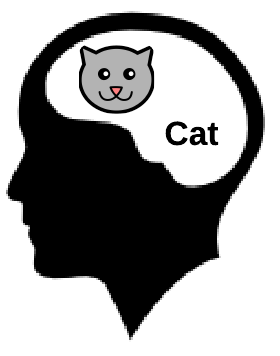
\includegraphics[scale=0.35]{pics/dualCoding.png}
    \end{center}
    \vspace{-20pt}
    \caption{Dual-Coding Theory}
    \vspace{-10pt}
  \end{wrapfigure}

  In many years, the field of psychology been a important in order to understand how humans interpret and remember different information. Psychology studies have recognized that the human brain have a superior memory for recognizing and recalling visual information rather than recognizing and recalling verbal or textual information \cite{DeAngeli}. One known theory is the ``dual-coding theory'' \cite{Biddle}, suggesting that verbal and non-verbal memory are processed and represented differently in humans mind. Text are verbal information that is represented symbolically, in contrast to non-verbal information like images that are mentally represented in a way that perceived concepts are assigned to a perceived meaning of what is directly observed. Both verbal and non-verbal information can be used when recalling information. For example, say a person have received stimulus of the concept ``cat'', both the image of a cat as well as the word ``cat''. When the person is asked to recall the concept ``cat'', the person can retrieve the image or the word individually, or both simultaneously. If the word ``cat'' is recalled, the image of the cat is not lost and can still be retrieved at a later point in time. The ability to code a stimulus in two different ways can increase humans ability to remember, in contrast to only code the stimulus in one way. In the background theory there are described three different categories of graphical passwords according to the memory task involved in remembering and entering the password, e.g. recall, recognition and cued-recall. 

  When it comes to humans and visual interpretation, studies supports the idea that people recall symmetric images better than asymmetric images \cite{Attneave, French}. A particular interesting observation is that mirror symmetry carries a special status i the human memory\cite{Wagemans}. A understanding of psychological studies on humans visual memory can help to build successfully attacks against graphical passwords. If an attacker can successfully use the symmetric properties of graphical password schemes, then the security may be significantly less than if all passwords were equivalent probable. 

  Humans do not only tend to choose symmetric passwords, but do also tend to be influenced by the graphical elements in a password scheme. A study on ``PassFace'' \cite{Davis} showed that there was a high bias in the password selection according to a users demography. When they analyzed how each gender choose their password, the most of the male and female participants chose female faces, and and 60-70\% of the user chose a model over a typical female/male. They also looked into the race of the faces, where the results showed that almost all of the participant chose their own race. 

  There is a lot of studies on password based on psychology and human factors, but the graphical passwords schemes being analyzed do not look at the background of the users. Humans are different in terms of their demographics, like gender, age and culture in their country. Analysis of people choices of graphical password based on users background have not been looked further into in published reseach as based on this state of the art research. 


  {\bf \color{red} Legge til mer forskning}

  {\bf \color{red} Studere papers fra Thorpe and Van Oorschot}
  

\section{Graphical Passwords and Mobile Devices}
  %Intro
  Users are not only dependent on remembering passwords across multiple web pages and systems, but do also need to remember passwords for our small mobile devices. The mobile phone have emerged as a good platform for graphical passwords because it is easier to input on touchscreen as a contrast to text-based passwords. Graphical passwords on mobile devices seems as a natural fit, as they often require direct manipulation of visual elements. In todays society we're addicted to our mobile devices in our every day life. Mobile devices are not just a communication tool for calling and texting, but also an important tool for every day tasks like doing our work, reading mail, pay our bills and keeping up with our social life. This trend makes our mobile devices vulnerable in terms of security. To avoid unwanted access, smartphones offers different locking mechanisms. The history of locking mechanisms was often a solution solely to prevent accidental use, while current mobile phones require protection in order to secure the potentially vast amount of private data that we keep on our smartphones. Our mobile devices are in rapidly use, as well as it well suited platform for graphical password, makes authentication on mobile devices an interesting field of study.

  {\bf \color{red} Skrive om forskning som jeg har funnet. God overgang til neste kapittel?} 

  % The time used on unlocking the phone
  In terms of security it is interesting to look at the use of mobile devices and look at the locking habits among users on mobile devices. It is known that services that are rapidly used have weaker password because of the overhead the user needs to spend on typing their password. In 2014 a group of researchers published a field study of smartphone (un)locking behavior \cite{habits3}. Some of the problems with smartphone users tends to be their rapidly use of their phone. When the device are rabidly use, it results in a lot of time unlocking their phone between every use. In the study they found that there was a significant overhead in the time used of unlocking their phone, where the users participated in the field study used 2.9\% (9\% in the worst case) of their time unlocking their smartphone. 

  It is important to understand why people use or not use locking mechanisms on their smartphone. Research have covered that the 46.8\% of the participants agreed or fully agreed that unlocking their phone can be annoying, but at the same time 95.5\% of the somewhat or fully agreed that they liked the idea that their phone was protected \cite{habits3}. This highlights that the users wants to be secure, but there might be a trade-off between the time used to unlock the smartphone vs the security risk.
  
  % The use of locking mechanisms
  Smartphones in use today do not require their users to have a locking mechanism on their smartphone. It is well known that users tends to choose to easiest way out and may result in the choice of not having any locking mechanism at all. Based on the result of the overhead in time used on unlocking their phone, a result may be to take the easiest way out by ignoring the vulnerability of not using a locking mechanism at all. It have been discovered that over 40\% of the users only used a basic ``slide-to-unlock'' mechanism on their smartphone, as well as over 16\% didn't use any locking mechanisms at all \cite{habits3}. This highlights a major bad habit among mobile users. What happens if your mobile is stolen? 

  % Risk vs securtiy
  One of the popular password schemes on mobile phones are the Android Unlock pattern. It is a graphical password that have been shown to have biases when the password are user-chosen. A research group did a large-scale user study on the Android Unlock Patterns in order to quantify its security \cite{Uellenbeck}. They analyses the biases introduced in the pattern making process and added changes to the scheme in order to avoid the known biases in the password scheme. The researchers found that there is a high bias in the pattern selection process, e.g. the upper left corner and three-point long straight lines are very typical selection strategies. If the patterns was uniformly chosen, the probability of starting in the top-left corner should be 11\%, but are instead close to 44\%. Another interesting result is the memorable password space used, where about 10\% of all users use less than 190 patterns, while less than 300 patterns capture around 50\% of the whole test population. This shows that a empirical password space are not a representative number when quantifying the security of a password, but we should look at the memorable password space, e.g. password that actually are used and memorable for the useres. The Android Unlock Patterns are a password scheme used on mobile devices. It is important to understand the difference of a password scheme used on a desktop vs. mobile device.

  The way that the mobile phone is held, the size of the screen may also impact the way that people write their passwords, but this may need further research to answer.
  
	\section{Discussion}

	{\bf \color{red} ** Oppsummere hva jeg har funnet og konkludere med hva som kan forskes videre på ***}

	%Bibtex
	\bibliographystyle{plain}
	\bibliography{myBib}

\end{document}